\documentclass[professionalfont,serif,german]{beamer}
\usepackage[utf8]{inputenc}
\usepackage[german]{babel}
\usepackage{xcolor}
\usetheme{Pittsburgh}
%\usetheme{Boadilla}

\usepackage{newtxtext,newtxmath}
\definecolor{pfblue}{RGB}{1, 0, 103}
\definecolor{pfred}{RGB}{255, 0, 86}
\definecolor{pfgreen}{RGB}{0, 255, 0}

\title[Pathfinder-Vergleicher]{Pathfinding-Algorithmen}
\subtitle{Einführung und Vergleich mittels einer Webapplikation}
\author[A. Stoop, S. Fürbringer]{Adrian Stoop und Severin Fürbringer}
\institute[BMZ, EVT18a]{Berufsmaturitätsschule Zürich \\ \tiny{Technik,
Architektur, Life Sciences}}
\date{5. März 2019}

%%%%%%%%%%%%%%%%%%%%%%%%%%%%%%%%%%%%%%%%%%%%%%%%%%%%%%%%%%%%%%%%%%%%%%%%%%%%%%%%

\begin{document}

\frame{\titlepage}

%%%%%%%%%%%%%%%%%%%%%%%%%%%%%%%%%%%%%%%%%%%%%%%%%%%%%%%%%%%%%%%%%%%%%%%%%%%%%%%%

\begin{frame}
  \frametitle{Inhalt}
  \tableofcontents
\end{frame}


%%%%%%%%%%%%%%%%%%%%%%%%%%%%%%%%%%%%%%%%%%%%%%%%%%%%%%%%%%%%%%%%%%%%%%%%%%%%%%%%
% 
%       IDEAS
% 
%   1)  Einfach verständliches Inhaltsverzeichnis (Oberflächlich)
% 
%   2)  Was ist ein Algorithmus: Mit dem echten Leben verbundenes Beispiel
%       - Am besten mit Medien und/oder Publikum arbeiten
% 
%   3)  Was ist ein Pathfinder: Vorgehen wie 2)
%       - Bezug zum Oberthema MOBILITÄT
% 
%   4)  Ziel der Arbeit: 
%       - Ziel: Was wollten wir herausfinden; Wieso welche Pathfinder auch
%       erläutern; Hypothese darlegen
%       - Wie: Webapplikation (Pathfinder-Vergleicher)
%       - Wieso: Was macht unsere Webapplikation speziell. Evtl. Alternativen
%       zeigen
% 
%   5)  Eingesetzte Methoden (Webapplikation und statistische Auswertung): 
%       - Funktion der Webapplikation: Wie vergleicht die Webapp die
%       Pathfinder?
%       - Statistik: Wie haben wir die Daten erhoben und Ausgewertet?
%
%   6)  Demo der Webapplikation
%       - Teil evtl. zusammen mit der Klasse machen; Jeder kann die
%       Webapplikation auf seinem Handy aufrufen und kurz testen
%       - Parallel dazu eine Bedienungsanleitung
%
%   7)  Zusammenfassung:
%       [^ Bewertung on JP zur Hilfe nehmen, da mehrere Punkte hierzu
%       kritisiert wurden^]
%       - Resultate der Arbeit und statistischen Auswertung verständlich
%       erklären; Stellungnahme zur Hypothese mit Bezug zu den Resultaten
%       nehmen;
%       - Kurze Wiederholung was das ganze Resultat ist
%       - Erweiterungsmöglichkeiten und Schwachstellen
%       
%   8)  Schluss:
%       - Alle relevanten Links aufzeigen (Webapplikation-URL und
%       GitHub-Repository)
% 
%%%%%%%%%%%%%%%%%%%%%%%%%%%%%%%%%%%%%%%%%%%%%%%%%%%%%%%%%%%%%%%%%%%%%%%%%%%%%%%%

\begin{frame}
  \section[Einführung in Algorithmen und Pathfinder]{Einführung}
  \frametitle{Einführung}
  \framesubtitle{Was ist ein Algorithmus?}
  \begin{columns}[c] % the "c" option specifies center vertical alignment
    \begin{column}[T]{.5\textwidth} % column designated by a command
      \begin{itemize}
        \item \textbf{Plan zur Lösung eines Problems}
        \item Name abstammend von al-Chwarizmi (* 780, lt. Algorismi)
          % (lt. == latein) 
          % Al-Chwarizmi (Iraner)gilt als einer der bedeutendsten Mathematiker,
          % da er sich mit Algebra als elementarer Untersuchungsform
          % beschäftigte.  Er entwickelte sozusagen Algorithmen zur grafischen
          % lösung von linearen und quadratischen Gleichungen
        \item Bsp.: Kochrezept, Lösungsverfahren für lin. oder quad. Gleichungen
        \item Relevant in der Informatik
      \end{itemize}
    \end{column}
    \begin{column}[T]{.5\textwidth}
      \begin{figure}
        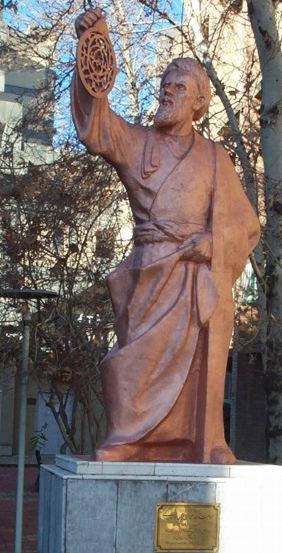
\includegraphics[height=4.5cm]{img/algorismi.png}
        \caption{Statue von al-Chwarizmi in Iran, Quelle: M. Tomczak, 2013}
      \end{figure}
    \end{column}
  \end{columns}
  % Evtl. hier Interaktion mit Publikum "Was ist euer Algorithmus um sich in
  % einer fremden Stadt zu orientieren?"
\end{frame}
\begin{frame}
  \frametitle{Einführung}
  \framesubtitle{Was sind Pathfinding-Algorithmen?}
  \begin{columns}
    \begin{column}[T]{.4\textwidth}
      \begin{itemize}
        \item \textbf{Finden den Weg von \texttt{A} nach \texttt{B}}
        \item Es gibt verschiedene Arten von Pathfinder
        \item Zentrale Rolle in dieser BMA
      \end{itemize}
    \end{column}
    \begin{column}[T]{.6\textwidth}
      \begin{figure}
        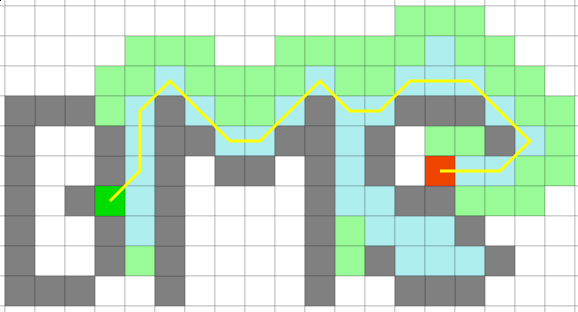
\includegraphics[height=3cm]{img/bms.png}
        \caption{BestFirstFinder findet den Weg (Grün ist Start, Rot ist Ende)}
      \end{figure}
    \end{column}
  \end{columns}
\end{frame}

\begin{frame}
  \frametitle{Einführung}
  \framesubtitle{Was hat das mit Mobilität zu tun?}
    Pathfinding-Algorithmen kommen vor in:
    \begin{columns}
      \begin{column}[T]{0.5\textwidth}
        \begin{itemize}
          \item Selbstfahrenden Fahrzeugen
          \item Digitalen Maps (Routenplanung)
          \item Netzwerktechnik
          \item Videospielen
        \end{itemize}
      \end{column}
      \begin{column}[T]{0.5\textwidth}
        \begin{figure}
          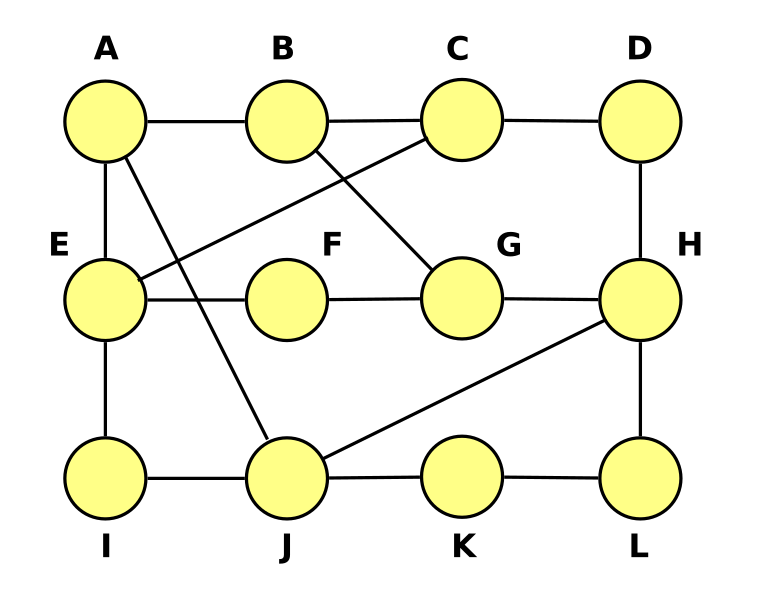
\includegraphics[height=3cm]{img/routing.png}
          \caption{Graph eines Computernetzwerks. Quelle: Wikibooks, 2008 (Public Domain)}
        \end{figure}
      \end{column}
    \end{columns}
\end{frame}

\begin{frame}
  \section{Produkt}
  \frametitle{Das Produkt}
    \begin{columns}
      \begin{column}[T]{0.5\textwidth}
        Pathfinding-Algorithmen brauchen einen Raum.
      \end{column}
      \begin{column}[T]{0.5\textwidth}
        \begin{figure}
          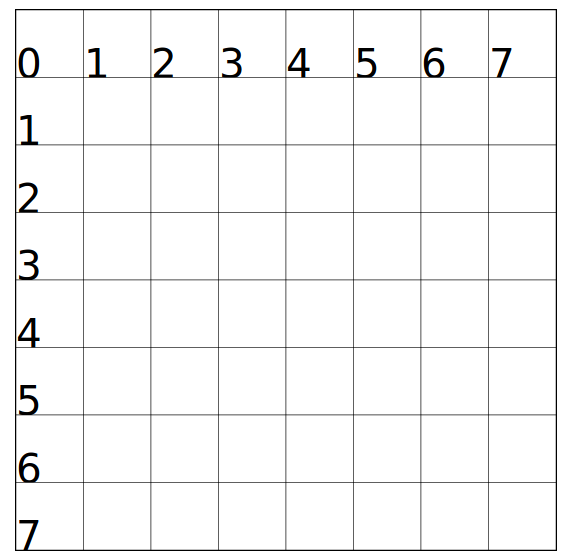
\includegraphics[height=4cm]{img/grid1.png}
        \end{figure}
      \end{column}
    \end{columns}
\end{frame}

\begin{frame}
  \frametitle{Das Produkt}
  \framesubtitle{Korridore und Wände}
  \begin{columns}
    \begin{column}[T]{0.5\textwidth}
      \begin{itemize}
        \item Leer $\rightarrow$ Korridor (passierbar)
        \item Grau $\rightarrow$ Wand
        \item Blau $\rightarrow$ Startpunkt
        \item Grün $\rightarrow$ Ziel
      \end{itemize}
    \end{column}
    \begin{column}[T]{0.5\textwidth}
      \begin{figure}
        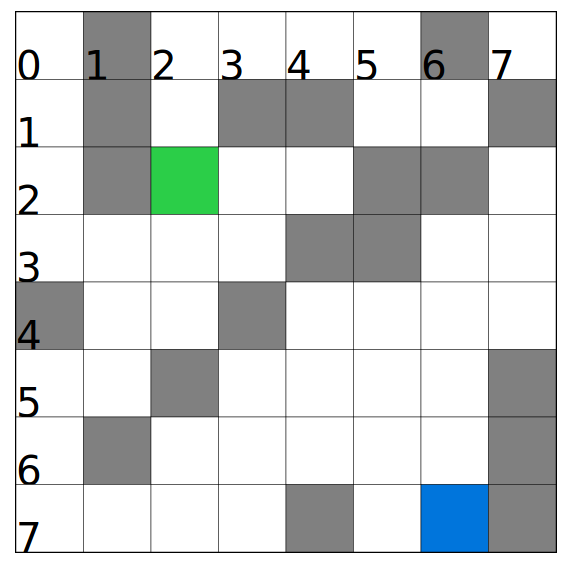
\includegraphics[height=4cm]{img/grid2.png}
      \end{figure}
    \end{column}
  \end{columns}
\end{frame}

\begin{frame}
  \frametitle{Das Produkt}
  \framesubtitle{Pathfinding-Algorithmen werden angewendet}
  \begin{columns}
    \begin{column}[T]{0.5\textwidth}
      \begin{itemize}
        \item Ausführung der drei ausgewählten Pathfinding-Algorithmen.
        \item \textcolor{pfblue}{A*}
        \item \textcolor{pfred}{BestFirstFinder}
        \item \textcolor{pfgreen}{BreadthFirstFinder}
      \end{itemize}
    \end{column}
    \begin{column}[T]{0.5\textwidth}
      \begin{figure}
        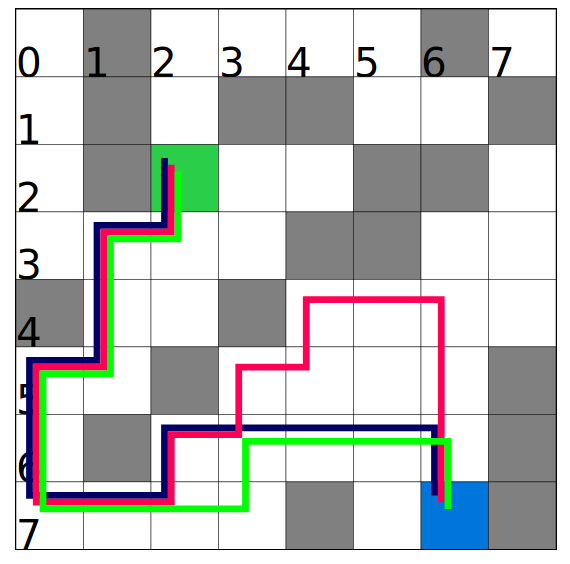
\includegraphics[height=4cm]{img/grid3.png}
      \end{figure}
    \end{column}
  \end{columns}
\end{frame}

\begin{frame}
  \section[Vielen Dank für eure Aufmerksamkeit!]{Schluss}
  \framesubtitle{Vielen Dank für eure Aufmerksamkeit!}
  \frametitle{Schluss}
  \begin{itemize}
    \item BMA-Produkt als Webapplikation:\\ \url{bma.fuerbringer.info}
    \item Quelltext Webapplikation und Dokument:\\
      \url{github.com/fuerbringer/bma}
  \end{itemize}
\end{frame}

\end{document}
